%% LyX 1.3 created this file.  For more info, see http://www.lyx.org/.
%% Do not edit unless you really know what you are doing.
\documentclass[english]{article}
\usepackage{pslatex}
\usepackage[T1]{fontenc}
\usepackage[latin1]{inputenc}
\usepackage{geometry}
\geometry{verbose,letterpaper,tmargin=10mm,bmargin=15mm,lmargin=10mm,rmargin=10mm}
\setcounter{secnumdepth}{4}
\setlength\parskip{\medskipamount}
\setlength\parindent{0pt}
\usepackage{color}
\usepackage{graphicx}

\makeatletter
%%%%%%%%%%%%%%%%%%%%%%%%%%%%%% Textclass specific LaTeX commands.
 \usepackage{verbatim}
 \newenvironment{lyxcode}
   {\begin{list}{}{
     \setlength{\rightmargin}{\leftmargin}
     \setlength{\listparindent}{0pt}% needed for AMS classes
     \raggedright
     \setlength{\itemsep}{0pt}
     \setlength{\parsep}{0pt}
     \normalfont\ttfamily}%
    \item[]}
   {\end{list}}

\AtBeginDocument{
  \renewcommand{\labelitemii}{\(\ast\)}
  \renewcommand{\labelitemiii}{\normalfont\bfseries{--}}
}

\usepackage{babel}
\makeatother
\begin{document}

\title{\textcolor{black}{Flowreplay Design Notes}}


\author{\textcolor{black}{Aaron Turner }\\
\textcolor{black}{http://synfin.net/}}


\date{\textcolor{black}{Last Edited:}\\
\textcolor{black}{October 23, 2003}}

\maketitle

\newpage
\section{\textcolor{black}{Overview}}

\textcolor{black}{Tcpreplay}%
\footnote{\textcolor{black}{http://tcpreplay.sourceforge.net/}%
} \textcolor{black}{was designed to replay traffic previously captured
in the pcap format back onto the wire for testing NIDS and other passive
devices. Over time, it was enhanced to be able to test in-line network
devices. However, a re-occurring feature request for tcpreplay is
to connect to a server in order to test applications and host TCP/IP
stacks. It was determined early on, that adding this feature to tcpreplay
was far too complex, so I decided to create a new tool specifically
designed for this.}

\textcolor{black}{Flowreplay is designed to replay traffic at Layer
4 or 7 depending on the protocol rather then at Layer 2 like tcpreplay
does. This allows flowreplay to connect to one or more servers using
a pcap savefile as the basis of the connections. Hence, flowreplay
allows the testing of applications running on real servers rather
then passive devices. }


\section{\textcolor{black}{Features}}


\subsection{\textcolor{black}{Requirements}}

\begin{enumerate}
\item \textcolor{black}{Full TCP/IP support, including IP fragments and
TCP stream reassembly.}
\item \textcolor{black}{Support replaying TCP and UDP flows.}
\item \textcolor{black}{Code should handle each flow/service independently.}
\item \textcolor{black}{Should be able to connect to the server(s) in the
pcap file or to a user specified IP address.}
\item \textcolor{black}{Support a plug-in architecture to allow adding application
layer intelligence.}
\item \textcolor{black}{Plug-ins must be able to support multi-flow protocols
like FTP.}
\item \textcolor{black}{Ship with a default plug-in which will work {}``well
enough'' for simple single-flow protocols like HTTP and telnet.}
\item \textcolor{black}{Flows being replayed {}``correctly'' is more important
then performance (Mbps).}
\item \textcolor{black}{Portable to run on common flavors of Unix and Unix-like
systems.}
\end{enumerate}

\subsection{\textcolor{black}{Wishes}}

\begin{enumerate}
\item \textcolor{black}{Support clients connecting to flowreplay on a limited
basis. Flowreplay would replay the server side of the connection.}
\item \textcolor{black}{Support other IP based traffic (ICMP, VRRP, OSPF,
etc) via plug-ins.}
\item \textcolor{black}{Support non-IP traffic (ARP, STP, CDP, etc) via
plug-ins.}
\item \textcolor{black}{Limit which flows are replayed using user defined
filters. (bpf filter syntax?)}
\item \textcolor{black}{Process pcap files directly with no intermediary
file conversions.}
\item \textcolor{black}{Should be able to scale to pcap files in the 100's
of MB in size and 100+ simultaneous flows on a P3 500MHz w/ 256MB
of RAM.}
\end{enumerate}

\section{\textcolor{black}{Design Thoughts}}


\subsection{\textcolor{black}{Sending and Receiving traffic}}

\textcolor{black}{Flowreplay must be able to process multiple connections
to one or more devices. There are two options:}

\begin{enumerate}
\item \textcolor{black}{Use sockets}%
\footnote{\textcolor{black}{socket(2)}%
} \textcolor{black}{to send and receive data}
\item \textcolor{black}{Use libpcap}%
\footnote{\textcolor{black}{http://www.tcpdump.org/}%
} \textcolor{black}{to receive packets and libnet}%
\footnote{\textcolor{black}{http://www.packetfactory.net/projects/libnet/}%
} \textcolor{black}{to send packets}
\end{enumerate}
\textcolor{black}{Although using libpcap/libnet would allow more simultaneous
connections and greater flexibility, there would be a very high complexity
cost associated with it. With that in mind, I've decided to use sockets
to send and receive data.}


\subsection{\textcolor{black}{Handling Multiple Connections}}

\textcolor{black}{Because a pcap file can contain multiple simultaneous
flows, we need to be able to support that too. The biggest problem
with this is reading packet data in a different order then stored
in the pcap file. }

\textcolor{black}{Reading and writing to multiple sockets is easy
with select() or poll(), however a pcap file has it's data stored
serially, but we need to access it randomly. There are a number of
possible solutions for this such as caching packets in RAM where they
can be accessed more randomly, creating an index of the packets in
the pcap file, or converting the pcap file to another format altogether.
Alternatively, I've started looking at libpcapnav}%
\footnote{http://netdude.sourceforge.net/%
} \textcolor{black}{as an alternate means to navigate a pcap file and
process packets out of order.}


\subsection{\textcolor{black}{Data Synchronization}}

\textcolor{black}{Knowing when to start sending client traffic in
response to the server will be \char`\"{}tricky\char`\"{}. Without
understanding the actual protocol involved, probably the best general
solution is waiting for a given period of time after no more data
from the server has been received. Not sure what to do if the client
traffic doesn't elicit a response from the server (implement some
kind of timeout?). This will be the basis for the default plug-in.}


\subsection{\textcolor{black}{TCP/IP}}

\textcolor{black}{Dealing with IP fragmentation and TCP stream reassembly
will be another really complex problem. We're basically talking about
implementing a significant portion of a TCP/IP stack. One thought
is to use libnids}%
\footnote{\textcolor{black}{http://www.avet.com.pl/\textasciitilde{}nergal/libnids/}%
} \textcolor{black}{which basically implements a Linux 2.0.37 TCP/IP
stack in user-space. Other solutions include porting a TCP/IP stack
from Open/Net/FreeBSD or writing our own custom stack from scratch.}


\section{\textcolor{black}{Multiple Independent Flows}}

\textcolor{black}{The biggest asynchronous problem, that pcap files
are serial, has to be solved in a scaleable manner. Not much can be
assumed about the network traffic contained in a pcap savefile other
then Murphy's Law will be in effect. This means we'll have to deal
with:}

\begin{itemize}
\item \textcolor{black}{Thousands of small simultaneous flows (captured
on a busy network)}
\item \textcolor{black}{Flows which {}``hang'' mid-stream (an exploit
against a server causes it to crash)}
\item \textcolor{black}{Flows which contain large quantities of data (FTP
transfers of ISO's for example)}
\end{itemize}
\textcolor{black}{How we implement parallel processing of the pcap
savefile will dramatically effect how well we can scale. A few considerations:}

\begin{itemize}
\item Most Unix systems limit the maximum number of open file descriptors
a single process can have. Generally speaking this shouldn't be a
problem except for highly parallel pcap's.
\item While RAM isn't limitless, we can use mmap() to get around this.
\item Many Unix systems have enhanced solutions to poll() which will improve
flow management.
\end{itemize}
\begin{comment}
\textcolor{black}{Unix systems implement a maximum limit on the number
of file descriptors a single process can open. My Linux box for example
craps out at 1021 (it's really 1024, but 3 are reserved for STDIN,
STDOUT, STDERR), which seems to be pretty standard for recent Unix's.
This means we're limited to at most 1020 simultaneous flows if the
pcap savefile is opened once and half that (510 flows) if the savefile
is re-opened for each flow.}%
\footnote{\textcolor{black}{It appears that most Unix-like OS's allow root to
increase the {}``hard-limit'' beyond 1024. Compiling a list of methods
to do this for common OS's should be added to the flowreplay documentation.}%
}

\textcolor{black}{RAM isn't limitless. Caching packets in memory may
cause problems when one or more flows with a lot of data {}``hang''
and their packets have to be cached so that other flows can be processed.
If you work with large pcaps containing malicious traffic (say packet
captures from DefCon), this sort of thing may be a real problem. Dealing
with this situation would require complicated buffer limits and error
handling.}

\textcolor{black}{Jumping around in the pcap file via fgetpos() and
fsetpos() is probably the most disk I/O intensive solution and may
effect performance. However, on systems with enough free memory, one
would hope the system disk cache will provide a dramatic speedup.
The {}``bookmarks'' used by fgetpos/fsetpos are just 64 bit integers
which are relatively space efficent compared to other solutions.}

\textcolor{black}{The other typical asynchronous issue is dealing
with multiple sockets, which we will solve via poll()}%
\footnote{\textcolor{black}{poll(2)}%
}\textcolor{black}{. Each flow will define a} \textcolor{black}{\emph{struct
pollfd}} \textcolor{black}{and the amount of time in ms to timeout.
Then prior to calling poll() we walk the list of flows and create
the array of pollfd's and determine the flow(s) with the smallest
timeout. A list of these flows is saved for when poll() returns. Finally,
the current time is tucked away and the timeout and array of pollfd's
is passed to poll().}

\textcolor{black}{When poll() returns, the sockets that returned ready
have their plug-in called. If no sockets are ready, then the flows
saved prior to calling poll() are processed.}

\textcolor{black}{Once all flows are processed, all the flows not
processed have their timeout decremented by the time difference of
the current time and when poll was last called and we start again.}
\end{comment}

\subsection{\textcolor{black}{IP Fragments and TCP Streams}}

\textcolor{black}{There are five major complications with flowreplay:}

\begin{enumerate}
\item \textcolor{black}{The IP datagrams may be fragmented- we won't be
able to use the standard 5-tuple (src/dst IP, src/dst port, protocol)
to lookup which flow a packet belongs to.}
\item \textcolor{black}{IP fragments may arrive out of order which will
complicate ordering of data to be sent.}
\item \textcolor{black}{The TCP segments may arrive out of order which will
complicate ordering of data to be sent.}
\item \textcolor{black}{Packets may be missing in the pcap file because
they were dropped during capture.}
\item \textcolor{black}{There are tools like fragrouter which intentionally
create non-deterministic situations.}
\end{enumerate}
\textcolor{black}{First off, I've decided, that I'm not going to worry
about fragrouter or it's cousins. I'll handle non-deterministic situations
one and only one way, so that the way flowreplay handles the traffic
will be deterministic. Perhaps, I'll make it easy for others to write
a plug-in which will change it, but that's not something I'm going
to concern myself with now.}

\textcolor{black}{Missing packets in the pcap file will probably make
that flow unplayable. There are proabably certain situation where
we can make an educated guess, but this is far too complex to worry
about for the first stable release.}

\textcolor{black}{That still leaves creating a basic TCP/IP stack
in user space. The good news it that there is already a library which
does this called libnids. As of version 1.17, libnids can process
packets from a pcap savefile (it's not documented in the man page,
but the code is there).}

\textcolor{black}{A potential problem with libnids though is that
it has to maintain it's own state/cache system. This not only means
additional overhead, but jumping around in the pcap file as I'm planning
on doing to handle multiple simultaneous flows is likely to really
confuse libnids' state engine. Also, libnids is licensed under the
GPL, but I want flowreplay released under a BSD-like license; I need
to research if the two are compatible in this way.}

\textcolor{black}{Possible solutions:}

\begin{itemize}
\item \textcolor{black}{Developing a custom wedge between the capture file
and libnids which will cause each packet to only be processed a single
time.}
\item \textcolor{black}{Use libnids to process the pcap file into a new
flow-based format, effectively putting the TCP/IP stack into a dedicated
utility.}
\item \textcolor{black}{Develop a custom user-space TCP/IP stack, perhaps
based on a BSD TCP/IP stack, much like libnids is based on Linux 2.0.37.}
\item \textcolor{black}{Screw it and say that IP fragmentation and out of
order IP packets/TCP segments are not supported. Not sure if this
will meet the needs of potential users.}
\end{itemize}

\subsection{\textcolor{black}{Blocking}}

\textcolor{black}{As earlier stated, one of the main goals of this
project is to keep things single threaded to make coding plugins easier.
One caveat of that is that any function which blocks will cause serious
problems.}

\textcolor{black}{There are three major cases where blocking is likely
to occur:}

\begin{enumerate}
\item \textcolor{black}{Opening a socket}
\item \textcolor{black}{Reading from a socket}
\item \textcolor{black}{Writing to a socket}
\end{enumerate}
\textcolor{black}{Reading from sockets in a non-blocking manner is
easy to solve for using poll() or select(). Writing to a socket, or
merely opening a TCP socket via connect() however requires a different
method:}

\begin{quotation}
\textcolor{black}{It is possible to do non-blocking IO on sockets
by setting the O\_NONBLOCK flag on a socket file descriptor using
fcntl(2). Then all operations that would block will (usually) return
with EAGAIN (operation should be retried later); connect(2) will return
EINPROGRESS error. The user can then wait for various events via poll(2)
or select(2).}%
\footnote{\textcolor{black}{socket(7)}%
}
\end{quotation}
\textcolor{black}{If connect() returns EINPROGRESS, then we'll just
have to do something like this:}

\begin{lyxcode}
\textcolor{black}{int~e,~len=sizeof(e);}

\textcolor{black}{if~(getsockopt(conn->s,~SOL\_SOCKET,~SO\_ERROR,~\&e,~\&len)~<~0)~\{~}

~\textcolor{black}{~~~/{*}~not~yet~{*}/}

~\textcolor{black}{~~~if(errno~!=~EINPROGRESS)\{~~/{*}~yuck.~kill~it.~{*}/~}

~\textcolor{black}{~~~~~~log\_fn(LOG\_DEBUG,\char`\"{}in-progress~connect~failed.~Removing.\char`\"{});~}

~\textcolor{black}{~~~~~~return~-1;~}

~\textcolor{black}{~~~\}~else~\{~}

~\textcolor{black}{~~~~~~return~0;~/{*}~no~change,~see~if~next~time~is~better~{*}/~}

~\textcolor{black}{~~~\}~}

\textcolor{black}{\}~}

\textcolor{black}{/{*}~the~connect~has~finished.~{*}/~}
\end{lyxcode}
\begin{quote}
\textcolor{black}{Note: It may not be totally right, but it works
ok. (that chunk of code gets called after poll returns the socket
as writable. if poll returns it as readable, then it's probably because
of eof, connect fails. You must poll for both.}
\end{quote}

\section{\textcolor{black}{pcap vs flow File Format}}

\textcolor{black}{As stated before, the pcap file format really isn't
well suited for flowreplay because it uses the raw packet as a container
for data. Flowreplay however isn't interested in packets, it's interested
in data streams}%
\footnote{\textcolor{black}{A {}``data stream'' as I call it is a simplex
communication from the client or server which is a complete query,
response or message.}%
} \textcolor{black}{which may span one or more TCP/UDP segments, each
comprised of an IP datagram which may be comprised of multiple IP
fragments. Handling all this additional complexity requires a full
TCP/IP stack in user space which would have additional feature requirements
specific to flowreplay.}

\textcolor{black}{Rather then trying to do that, I've decided to create
a pcap preprocessor for flowreplay called: flowprep. Flowprep will
handle all the TCP/IP defragmentation/reassembly and write out a file
containing the data streams for each flow.}

\textcolor{black}{A flow file will contain three sections:}

\begin{enumerate}
\item \textcolor{black}{A header which identifies this as a flowprep file
and the file version}
\item \textcolor{black}{An index of all the flows contained in the file}
\item \textcolor{black}{The data streams themselves}
\end{enumerate}
\begin{center}\textcolor{black}{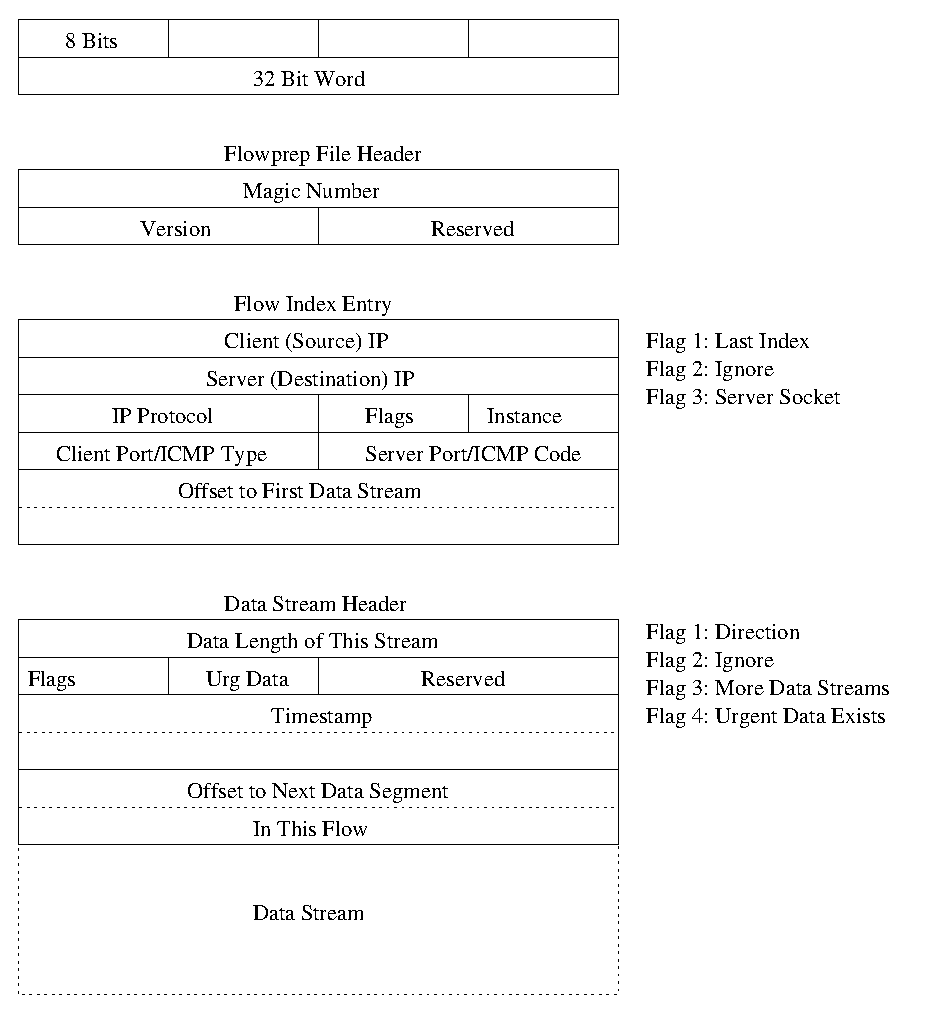
\includegraphics{flowheader.eps}}\end{center}

\textcolor{black}{At startup, the file header is validated and the
data stream indexes are loaded into memory. Then the first data stream
header from each flow is read. Then each flow and subsequent data
stream is processed based upon the timestamps and plug-ins.}


\section{\textcolor{black}{Plug-ins}}

\textcolor{black}{Plug-ins will provide the {}``intelligence'' in
flowreplay. Flowreplay is designed to be a mere framework for connecting
captured flows in a flow file with socket file handles. How data is
processed and what should be done with it will be done via plug-ins.}

\textcolor{black}{Plug-ins will allow proper handling of a variety
of protocols while hopefully keeping things simple. Another part of
the consideration will be making it easy for others to contribute
to flowreplay. I don't want to have to write all the protocol logic
myself.}


\subsection{\textcolor{black}{Plug-in Basics}}

\textcolor{black}{Each plug-in provides the logic for handling one
or more services. The main purpose of a plug-in is to decide when
flowreplay should send data via one or more sockets. The plug-in can
use any} \textcolor{black}{\emph{non-blocking}} \textcolor{black}{method
of determining if it appropriate to send data or wait for data to
received. If necessary, a plug-in can also modify the data sent.}

\textcolor{black}{Each time poll() returns, flowreplay calls the plug-ins
for the flows which either have data waiting or in the case of a timeout,
those flows which timed out. Afterwords, all the flows are processed
and poll() is called on those flows which have their state set to
POLL. And the process repeats until there are no more nodes in the
tree.}


\subsection{\textcolor{black}{The Default Plug-in}}

\textcolor{black}{Initially, flowreplay will ship with one basic plug-in
called {}``default''. Any flow which doesn't have a specific plug-in
defined, will use default. The goal of the default plug-in is to work
{}``good enough'' for a majority of single-flow protocols such as
SMTP, HTTP, and Telnet. Protocols which use encryption (SSL, SSH,
etc) or multiple flows (FTP, RPC, etc) will never work with the default
plug-in. Furthermore, the default plug-in will only support connections}
\textcolor{black}{\emph{to}} \textcolor{black}{a server, it will not
support accepting connections from clients.}

\textcolor{black}{The default plug-in will provide no data level manipulation
and only a simple method for detecting when it is time to send data
to the server. Detecting when to send data will be done by a {}``no
more data'' timeout value. Basically, by using the pcap file as a
means to determine the order of the exchange, anytime it is the servers
turn to send data, flowreplay will wait for the first byte of data
and then start the {}``no more data'' timer. Every time more data
is received, the timer is reset. If the timer reaches zero, then flowreplay
sends the next portion of the client side of the connection. This
is repeated until the the flow has been completely replayed or a {}``server
hung'' timeout is reached. The server hung timeout is used to detect
a server which crashed and never starts sending any data which would
start the {}``no more data'' timer.}

\textcolor{black}{Both the {}``no more data'' and {}``server hung''
timers will be user defined values and global to all flows using the
default plug-in.}


\subsection{\textcolor{black}{Plug-in Details}}

\textcolor{black}{Each plug-in will be comprised of the following:}

\begin{enumerate}
\item \textcolor{black}{An optional global data structure, for intra-flow
communication}
\item \textcolor{black}{Per-flow data structure, for tracking flow state
information}
\item \textcolor{black}{A list of functions which flow replay will call
when certain well-defined conditions are met.}

\begin{itemize}
\item \textcolor{black}{Required functions:}

\begin{itemize}
\item \textcolor{black}{initialize\_node() - called when a node in the tree
created using this plug-in}
\item \textcolor{black}{post\_poll\_timeout() - called when the poll() returned
due to a timeout for this node}
\item \textcolor{black}{post\_poll\_read() - called when the poll() returned
due to the socket being ready}
\item \textcolor{black}{buffer\_full() - called when a the packet buffer
for this flow is full}
\item \textcolor{black}{delete\_node() - called just prior to the node being
free()'d}
\end{itemize}
\item \textcolor{black}{Optional functions:}

\begin{itemize}
\item \textcolor{black}{pre\_send\_data() - called before data is sent}
\item \textcolor{black}{post\_send\_data() - called after data is sent}
\item \textcolor{black}{pre\_poll() - called prior to poll()}
\item \textcolor{black}{post\_poll\_default() - called when poll() returns
and neither the socket was ready or the node timed out }
\item \textcolor{black}{open\_socket() - called after the socket is opened}
\item \textcolor{black}{close\_socket() - called after the socket is closed}
\end{itemize}
\end{itemize}
\end{enumerate}
\begin{lyxcode}


\end{lyxcode}

\end{document}
